\section{Design}
\label{sec:design}
\paragraph{High level design}
Tracer is a designed as a generic pluggable tool for monitoring object level accesses for C programs. The high level design of Tracer can be bifurcated into two major components. These consist of an {\emph{interception}} based pre processing engine and a {\emph{monitoring engine}} coupled with the standard memory management library ({\emph{malloc library}}. Besides, Tracer provides flexible interfaces to the developer to monitor object access levels accurately. 

\paragraph{Flow of operations}
The flow of operations which eventually leads to memory monitoring can be summarized in the following three steps (refer to Fig. \ref{fig:architecture}):
\begin{enumerate}
\item A preprocessing engine which instruments C code with memory access calls.
\item A set of standard APIs which provide interfaces which:
\begin{itemize}
\item allocate/deallocate objects augmented with headers, 
\item register memory access calls
\item output summary of memory access footprint at object level granularity
\end{itemize}
\item A statistics store for saving application's object access count information.
\end{enumerate}

\begin{figure}[!ht]
\caption{High level architectural design}
\label{fig:architecture}
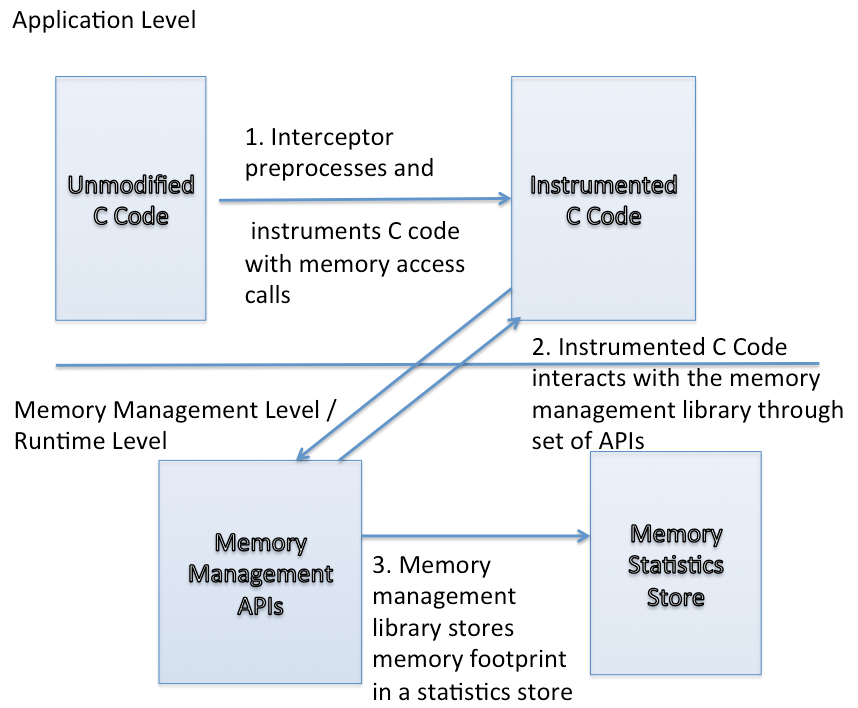
\includegraphics[scale=0.3]{./images/architecture.png}
\end{figure}

\paragraph{Interceptor: Transparent Instrumentation}
The interceptor uses preprocessing and code level instrumentation for injecting calls which enable the monitoring mechanism. In order to monitor object references, Tracer uses an interceptor which pre-processes standard C source code. The interceptor classifies literals into different classes of 8 different class types. {\emph{Identifiers}} which are allocated as dynamic objects are identified as {\emph{trace targets}}.  The interceptor adds an {\emph{access}} function call ({\emph{mem\_access}}) following an access to each {\emph{trace target}}. This {\emph{mem\_access}} library call increments the object's hidden count variable by one. 
\paragraph{Header Augmented Objects}
Tracer implements a custom version of the standard malloc library function named "{\emph{hmalloc}}" (header memory allocator) which {\emph{transparently}} inserts the target object with header field. The header acts as custom metadata store for the object. The design philosophy behind augmenting objects with headers is to be able to support faster updates. Our earlier design was plagued by the heavy overheads involved in looking up each objects counter within a hash table. {\emph{Object headers}} provide a clean solution to this problem since the metadata is now tagged to each object in memory. {\emph{Hmalloc}} function increases the amount of bytes requested by the size of an int, and uses the additional 4 bytes allocated to store the object count. A pointer to the memory location immediately following these four bytes, is then returned to the requesting program. These objects are then added to an object list that Tracer manages. It is a part of memory statistics interfaces (described in the next paragraph).
\paragraph{Memory Statistics Interfaces}
We provide the following interfaces to the application developer for getting memory statistics:
\begin{enumerate}
\item {\emph{void * hmalloc (size\_t bytes)}} - This interface allocates "bytes" size object tagged with a header
\item {\emph{void mem\_access\_stat}} - This interface prints the access count of all the objects allocated by the current program
\item {\emph{void hfree}} - frees objects tagged with headers
\item{\emph{void mem\_access(void *memory\_location, int count)}} - This interface increases the access count of the object at the memory location (memory\_location) by the count. This is the interface which is used by the memory interceptor to monitor object level access count
\item {\emph{int mem\_access\_count(void *object\_address)}} - This interface returns the current access count of the object (at memory location object\_address).
\end{enumerate}
